% --
% Neural Network Architectures

\section{Neural Network Architectures}\label{sec:nn_arch}
\thesisStateNotReady
All neural network architectures evaluated within this thesis are presented here.
The fundamental architectures were:
\begin{enumerate}
	\item Convolutional Neural Networks (CNN)
	\item Generative Adversarial Neural Networks (GAN)
	\item Wavenets
\end{enumerate}
%The term convolutional neural network here consists of all architectures consisting of at least one convolutional layer and the intention to simply classify each speech commands from each other. 
%Therefore the output of a convolutional net is of size of the number of individual speech commands and usually has some kind of probability distribution or energy equivalence.
CNNs were used for the classification of MFCC features and are therefore the main architecture within this thesis.
Generative models, such as GANs, are always worth to examine.
In this thesis, GANs were applied to evaluate network designs and their capability to generative convincing fakes and to use the trained feature maps in the convolutional layers for classifier networks as pre-trained weights.
Wavenets are compared to CNNs a completely different approach and use even raw audio samples as inputs.
Therefore for an online system, no MFCC features have to be calculated.
The saving of computations is evaluated as well as the performance compared to the CNN approach.

% --
% CNNs

\subsection{Convolutional Neural Networks}\label{sec:nn_arch_cnn}
Three different CNN designs were evaluated, with the focus of the striding properties and therefore also the sizes of convolutional filters.
For one model the kernel size has the length of the frame (time) dimension of the input features and is therefore striding only in the MFCC (frequency) dimension.
The same holds for another model, but so that the kernel has the size of the feature dimension and therefore strides only in the frame dimension.
Also one traditional model is used, that does the strides as usual in both dimensions.
The naming of those models is as following:
\begin{itemize}
	\item \enquote{\texttt{conv-trad}}: from \cite{Sainath2015} a traditional CNN network, striding in both dimensions.
	\item \enquote{\texttt{conv-fstride4}}: from \cite{Sainath2015}, striding only in frequency dimension.
	\item \enquote{\texttt{conv-jim}}: self designed model, striding only in frame dimension.
\end{itemize}
The naming of the \texttt{conv-trad} and \texttt{conv-fstride4} comes from their original papers, the self defined network \texttt{conv-jim} was named bluntly after the astronaut avatar shown inside this thesis very often.
The network architecture of the traditional network (\texttt{conv-trad}) is shown in \rfig{nn_arch_cnn_trad}.
% conv-trad
\begin{figure}[!ht]
  \centering
    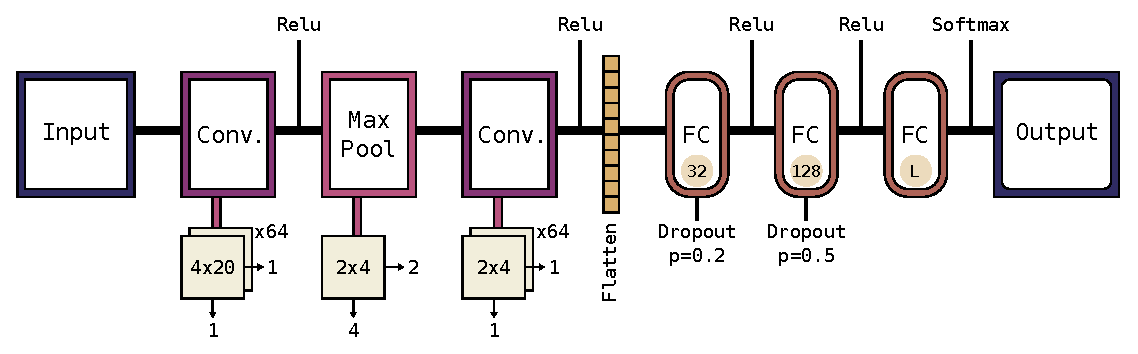
\includegraphics[height=0.2\textwidth]{./4_nn/figs/nn_arch_cnn_trad.eps}
  \caption{Traditional CNN network design from \cite{Sainath2015} named \texttt{conv-trad}.}
  \label{fig:nn_arch_cnn_trad}
\end{figure}
\FloatBarrier
\noindent
The \texttt{conv-trad} network consists of 2 convolutional layers and one max pooling layer in between.
The architecture was adapted from \cite{Sainath2015} as a baseline network and modified a bit in the kernel sizes, so that also reduced input features, for instance 12 MFCCs instead of 39 MFCC plus deltas and energies, can be computed with the same model.
The length of 20 frames in the first convolutional layer is reasonable and corresponse approximately to the length of a vowel sound.
Note that the \enquote{Flatten} layer simply flattens the output tensor of the last convolutional layers to 1-dimension, so that fully conected layers can be appended.
Dropout was used in the first two FC layers.
The last FC layer has $C$ nodes corresponding to $C$ output class labels, depending on the amount of chosen key words in the vocabulary.
Assuming that the input will be of shape $x = (1 \times 12 \times 50)$ this will give following dimensions and operations as listed in \rtab{nn_arch_cnn_trad}.
\begin{table}[ht!]
\small
\begin{center}
\caption{Network footprint of \texttt{conv-trad} with 12 output labels.}
\begin{tabular}{ M{1.5cm} M{1.4cm} M{1.2cm} M{1.2cm} M{2cm} M{1.8cm} M{2.3cm} }
\toprule
 \textbf{layer types} & \textbf{number of feature maps} & \textbf{kernel size} & \textbf{stride} & \textbf{output dimension} & \textbf{number of parameters} & \textbf{number of operations}\\
\midrule
input & - & - & - & $1 \times 12 \times 50$ & - & -\\
conv. & 64 & $(4 \times 20)$ & $(1, 1)$ & $64 \times 9 \times 31$ & \num{5184} & \SI{2874.82}{\kilo\ops}\\
max pool & - & $(2 \times 4)$ & $(2, 4)$ & $64 \times 4 \times 7$ & - & -\\
conv. & 64 & $(2 \times 4)$ & $(1, 1)$ & $64 \times 3 \times 4$ & \num{32832} & \SI{835.58}{\kilo\ops}\\
flatten & - & - & - & $1 \times 768$ & - & - \\
fc & - & - & - & $1 \times 32$ & \num{24608} & \SI{49.18}{\kilo\ops} \\
fc & - & - & - & $1 \times 128$ & \num{4224} & \SI{8.32}{\kilo\ops} \\
fc & - & - & - & $1 \times 12$ & \num{1548} & \SI{3.08}{\kilo\ops} \\
\midrule
\textbf{sum} & - & - & - & - & \textbf{\num{68396}} & \textbf{\SI{3770.98}{\kilo\ops}} \\ 
\bottomrule
\label{tab:nn_arch_cnn_trad}
\end{tabular}
\end{center}
\vspace{-4mm}
\end{table}
\FloatBarrier
\noindent

The \texttt{conv-fstride4} model is shown in \rfig{nn_arch_cnn_fstride}
\begin{figure}[!ht]
  \centering
    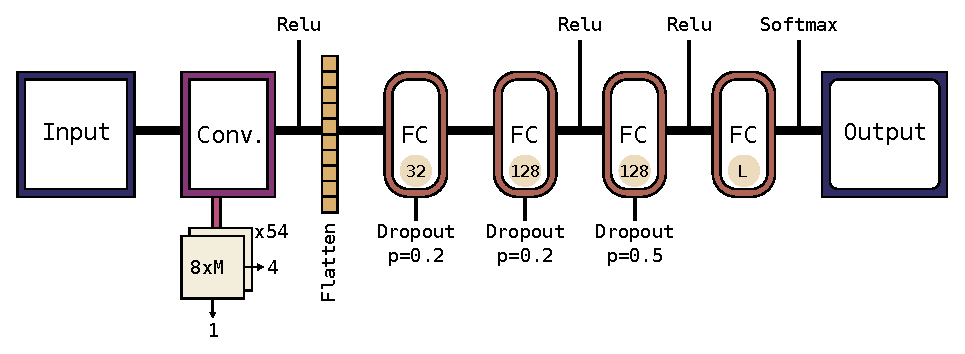
\includegraphics[height=0.2\textwidth]{./4_nn/figs/nn_arch_cnn_fstride.eps}
  \caption{Frequency striding CNN network design from \cite{Sainath2015} named \texttt{conv-fstride4}.}
  \label{fig:nn_arch_cnn_fstride}
\end{figure}
\FloatBarrier
\noindent

The self designed \texttt{conv-jim} model is shown in \rfig{nn_arch_cnn_conv-jim}.
\begin{figure}[!ht]
  \centering
    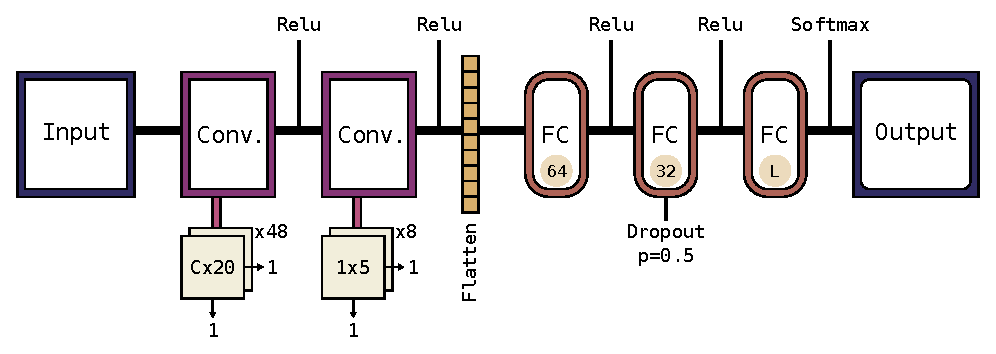
\includegraphics[height=0.2\textwidth]{./4_nn/figs/nn_arch_cnn_conv-jim.eps}
  \caption{Self designed frame (time) striding CNN named \texttt{conv-jim}.}
  \label{fig:nn_arch_cnn_conv-jim}
\end{figure}
\FloatBarrier
\noindent


% --
% GANs

\subsection{Adversarial Neural Networks}\label{sec:nn_arch_adv}
Generative Adversarial Neural Networks (GAN), as already mentioned in \rsec{prev_nn_adv} are consisting of two neural network architectures competing against each other.
The architectures are denoted as Discriminator (D) and Generator (G) network.
The G network is able to produce samples from the data distribution, while the D network has the role of discriminating between fake and real.
Being able to transfer the obtained weights from the training of the adversarial models, the layers parameters of the target network must coincide with the adversarial network layers.
Both D and G network convolutional layer parameters can be used, even if G performs a convolutional upsampling (transposed convolution) instead of usual convolution.

The major model tested with adversarial training has the same structure as the \texttt{conv-jim} network and is therefore denoted as \texttt{adv-d-jim} shown in \rfig{nn_arch_adv_d_jim} and \texttt{adv-g-jim} in \rfig{nn_arch_adv_g_jim}.

\begin{figure}[!ht]
  \centering
    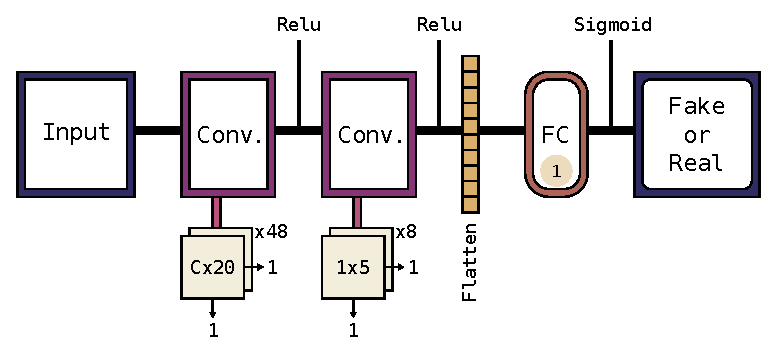
\includegraphics[height=0.2\textwidth]{./4_nn/figs/nn_arch_adv_d_jim.eps}
  \caption{Discriminator network named \texttt{adv-d-jim}.}
  \label{fig:nn_arch_adv_d_jim}
\end{figure}
\FloatBarrier
\noindent

\begin{figure}[!ht]
  \centering
    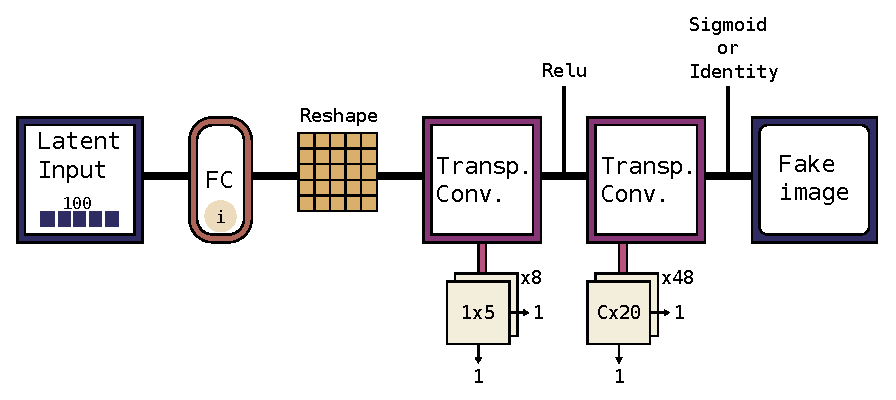
\includegraphics[height=0.23\textwidth]{./4_nn/figs/nn_arch_adv_g_jim.eps}
  \caption{Generator network named \texttt{adv-g-jim}.}
  \label{fig:nn_arch_adv_g_jim}
\end{figure}
\FloatBarrier
\noindent

%An overview of all models is shown in \rtab{nn_arch_overview} with abbreviations in \rtab{nn_arch_abbreviation}.
%\begin{table}[ht!]
\begin{center}
\caption{Network Architectures Abbreviations}
\begin{tabular}{ M{2.5cm}  M{10cm} }
\toprule
\textbf{Abbreviations} & \textbf{Meaning}\\
\midrule
c[0-9] & convolutional layer with layer number\\
f[0-9] & feed forward fully connected layer with layer number\\
m[0-9] & max pooling layer layer with layer number\\
ch & input channel number for mfccs it is usually 1\\
fs & frame size (usually 50 -> 50ms)\\
ms & feature size (mfcc), depends on feature selection\\
cf & output number of last flattened convolutional layer\\
cl & number of class labels\\
\bottomrule
\label{tab:nn_arch_abbreviation}
\end{tabular}
\end{center}
\vspace{-4mm}
\end{table}
\FloatBarrier
\noindent
%\begin{table}[ht!]
\begin{center}
\caption{Network Architectures Overview with reference names}
\begin{tabular}{ M{2.5cm}  M{2.1cm}  M{2.1cm} M{2.1cm} M{2.5cm}}
\toprule
%\multicolumn{4}{c}{\textbf{Feature Groups}} & \multicolumn{2}{c}{\textbf{Accuracy}} \\
\textbf{Reference name} & \textbf{Feature maps} & \textbf{Kernel sizes} & \textbf{Strides} & \textbf{Feed Forward} \\
\midrule
conv-trad & c1: (ch, 64) c3: (64, 64) & c1: (4, 20) m2: (2, 4) c3: (2, 4) & c1: (1, 1) m2: (2, 4) c3: (1, 1) & f4: (cf, 32) \quad f5: (32, 128) f6: (128, cl)\\
\midrule
conv-fstride & c1: (ch, 54) & c1: (8, fs) & c1: (4, 1) & f2: (cf, 32) \quad f3: (32, 128) \quad f4: (128, 128) \quad f5: (128, cl)\\
\midrule
conv-encoder-fc1 & c1: (ch, 48) \quad c2: (48, 8) & c1: (ms, 20) \quad c2: (1, 5) & c1: (1, 1) \quad c2: (1, 1) & f3: (cf, cl)\\
\midrule
conv-encoder-fc3 & c1: (ch, 48) \quad c2: (48, 8) & c1: (ms, 20) \quad c2: (1, 5) & c1: (1, 1) \quad c2: (1, 1) & f3: (cf, 64) \quad f4: (64, 32) \quad f5: (32, l)\\
\midrule
adv-d-label & c1: (ch, 8) \quad c2: (8, 8) & c1: (ms, 20) \quad c2: (1, 5) & c1: (1, 1) \quad c2: (1, 1) & f3: (cf, 1)\\
\midrule
adv-g-label & c2: (8, 8) \quad c3: (8, ch) & c2: (1, 5) \quad c3: (ms, 20) & c2: (1, 1) \quad c3: (1, 1) & f1: (100, cf)\\
\bottomrule
\label{tab:nn_arch_overview}
\end{tabular}
\end{center}
\vspace{-4mm}
\end{table}
\FloatBarrier
\noindent


% --
% wavenets
\subsection{Wavenets}\label{sec:nn_arch_wavenet}

A Wavenet residual block introduced by \cite{Oord2016}, with an extension for class prediction is illustrated in \rfig{nn_arch_wavenet_block} 
\begin{figure}[!ht]
  \centering
    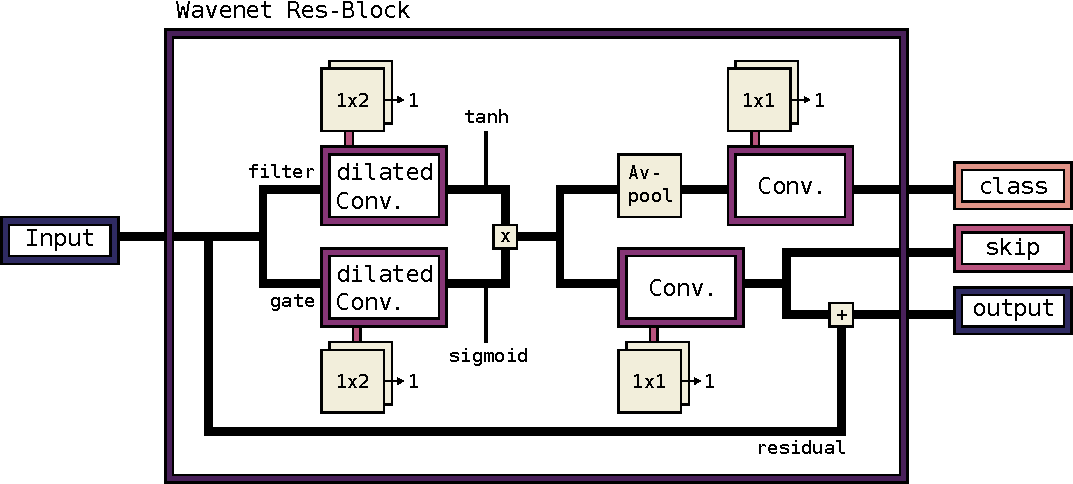
\includegraphics[width=0.7\textwidth]{./4_nn/figs/nn_arch_wavenet_block.eps}
  \caption{Wavenet residual block \cite{Oord2016} with extension of class prediction layers.}
  \label{fig:nn_arch_wavenet_block}
\end{figure}
\FloatBarrier
\noindent
The whole Wavenet architecture with class and sample prediction is shown in \rfig{nn_arch_wavenet_all}.
\begin{figure}[!ht]
  \centering
    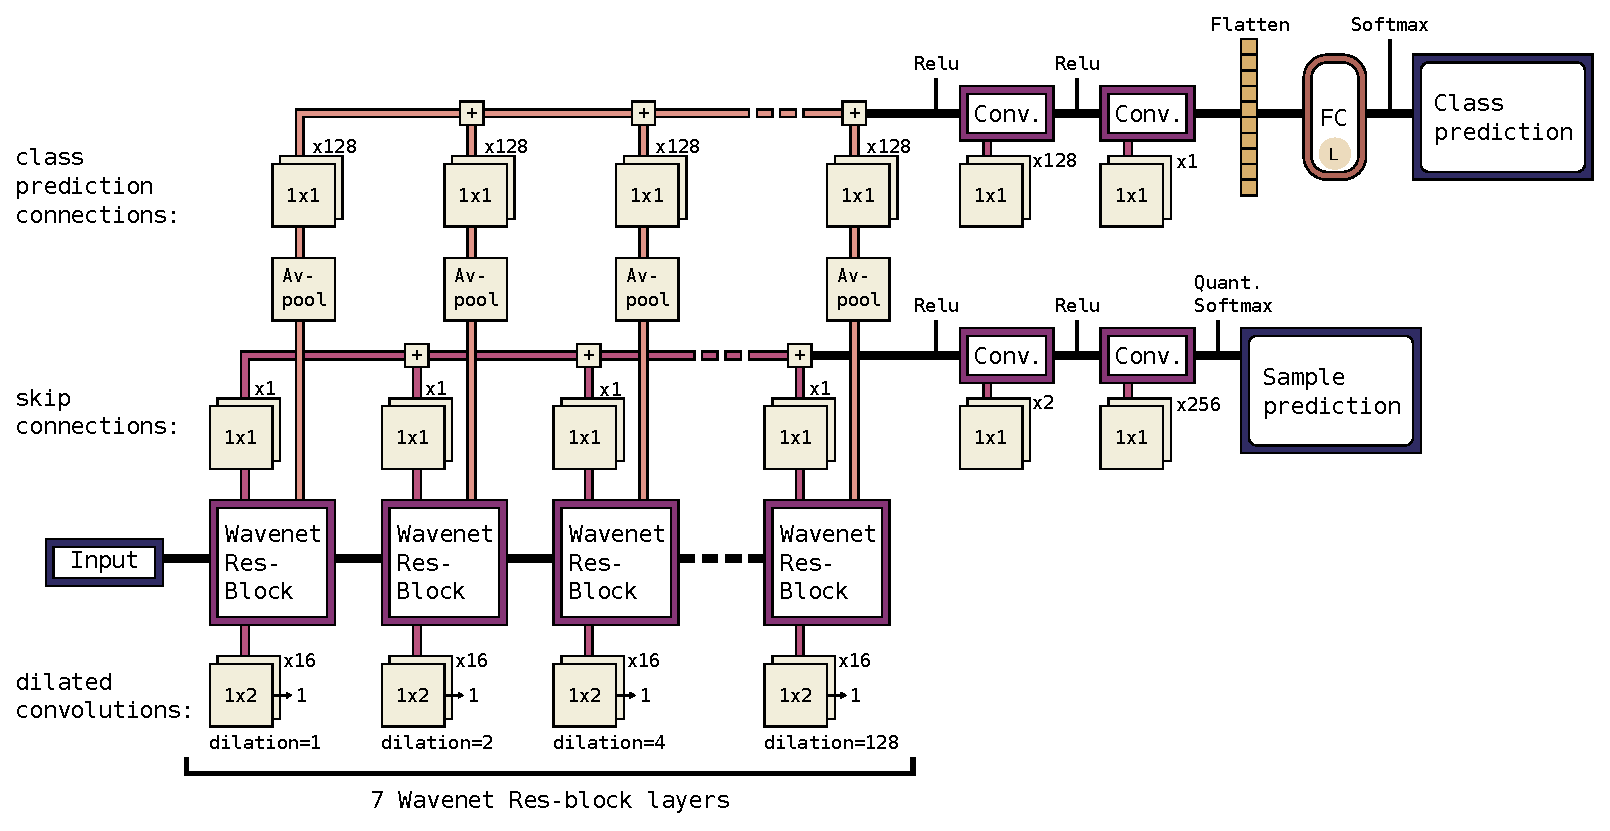
\includegraphics[width=0.9\textwidth]{./4_nn/figs/nn_arch_wavenet_all.eps}
  \caption{Wavenet architecture with class prediction extension.}
  \label{fig:nn_arch_wavenet_all}
\end{figure}
\FloatBarrier
\noindent

